\documentclass{article}

\usepackage{amsfonts}
\usepackage[colorlinks=true,citecolor=blue,urlcolor=cyan,linkcolor=red]{hyperref}
\usepackage{amssymb}
\usepackage{amsmath,amssymb,amscd,epsfig,amsfonts,rotating}
\usepackage{graphicx}
\usepackage{epsfig}
\usepackage{multirow}
\usepackage{booktabs}
\usepackage{url}
\usepackage[margin=1.5in]{geometry}

\newtheorem{def:def}{Definition}
\newtheorem{thm:thm}{Theorem}
\newtheorem{thm:lm}{Lemma}

\DeclareMathOperator*{\argmax}{arg \, max}
\DeclareMathOperator*{\var}{var}
\DeclareMathOperator*{\cov}{cov}
\newcommand{\bs}{\boldsymbol}

\title{An End-to-end solution for Semantic Modeling \\
		\Large{CS420 Coursework: Text Classification}}
\author{Author\\
{\small Kaggle Account, Student ID} \\
{\small Shanghai Jiao Tong University}\\
{\small \textsf{name@domain}}}
\begin{document}
\maketitle

\begin{abstract}
This note is a complementary material for the solution of coursework, add your abstract here.
You'd better summarize the methodology of your solution and declare the overall performance of your models.
\end{abstract}

\section{Introduction}\label{sec:intro}
\subsection{Background}\label{sec:bg}
Please describe the background information of this task.

\begin{table}
\small
\renewcommand{\arraystretch}{1}
\centering
\caption{Notations and descriptions}\label{tab:notation}
\resizebox{0.8\columnwidth}{!}{
\begin{tabular}{c|l}
\hline
Notation & Description \\
\hline
$\bs{x}$ & The pre-defined value of positive user response. \\
$y$ & The true label of user response. \\
$L(\bs{x})$ & The loss function of the objective.\\
$p$ & The predicted probability $Pr(\hat{y}=1|\bs{x})$.\\
\hline
\end{tabular}
}
\end{table}

\subsection{Formulation}\label{sec:formulate}
Please formulate the task and declare some preliminaries across the paper.
First you may present the notations with descriptions of your paper to improve the readability as that in Table~\ref{tab:notation}.
Then you can formally define the objective function and the problem in this part.

\section{Methodology}\label{sec:method}
Please describe your solution details in this section.
You may use the notations presented in Section.~\ref{sec:formulate}.
In this part, you'd better state these things clearly:
\begin{itemize}
	\item The model you used in your solution, including the objective function, e.g., Eq.~\ref{eq:loss} and the corresponding ideas.
	\item The optimization details, e.g., gradients of SGD\footnote{We refer SGD as stochastic gradient descent, against batch gradient descent.} or other methods.
	\item The modification you made in the original model. Note that, please also add the reference below of the cited paper, just like \cite{zhang2014optimal}. As for references, please search the paper in Google Scholar and paste the bibtex code in the \textit{.bib} file.
	\item Other thoughts of your methodology.
\end{itemize}

\begin{equation}\label{eq:loss}
	L(\bs{x}) = - \int_{\bs{x}} [y \log{p} + (1-y) \log{(1-p)}] d\bs{x} .
\end{equation}

\section{Experiments and Results}\label{sec:exps}
Please describe your experimental settings and the corresponding results in this section.
There are several things your need to state clearly.
\begin{itemize}
	\item Data preparation for your exps, e.g., partition of training/evaluation/test data, data preprocessing and feature engineering.
	\item (optional) Statistics about the your data.
	\item The evaluation metrics and the experimental results, with some discussions.
\end{itemize}
Note that we prefer \textit{.pdf} quality figures in the paper just like \ref{fig:basic}.
I have put a plotting script in the \textit{../code/} folder and you may run with your command line tools.

\begin{figure}[t]
  \centering
  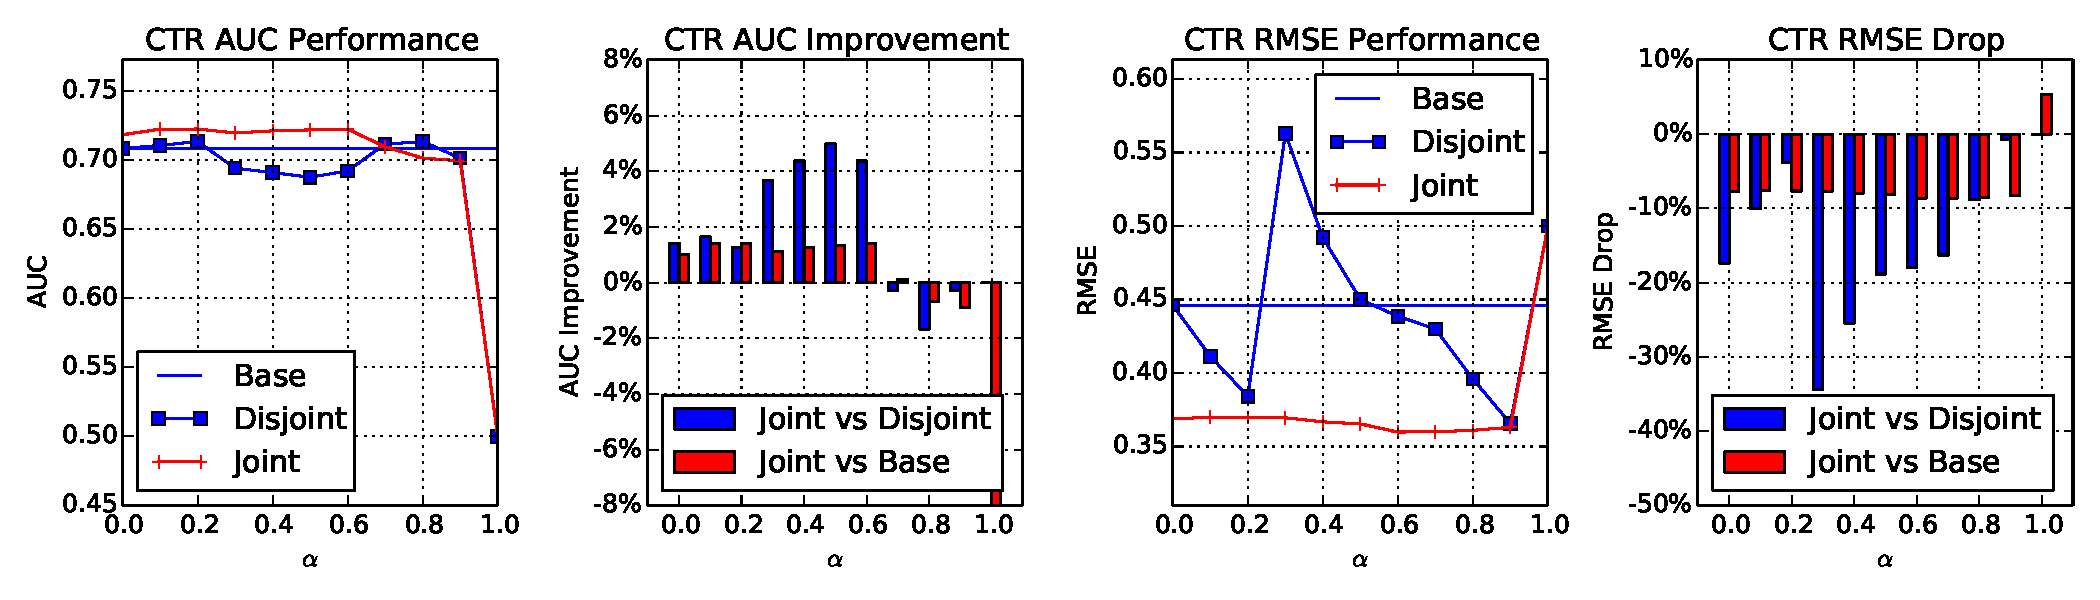
\includegraphics[width=1.0\columnwidth]{figures/basic-perf4.pdf}
  \caption{The illustration of the performance.}\label{fig:basic}
\end{figure}

\section{Discussion and Future works}\label{sec:discuss}
In this part, you may make some discussion about your solution and this problem.
Moreover, you are encouraged to think deeper in more general cases to find some future works about this direction.

\bibliographystyle{abbrv}
\bibliography{report}


\end{document}
